\section{Optimizations}

\TODO{This section needs a better name!}
\subsection{Notation}
\TODO{Notation needs to be introduced in the background section}
We represent a decision tree by $T = (V, E, r)$ where $V$ is the set of nodes, $E$ the set of edges and
$r \in V$ is the root. For each node $n \in V$, the following are given.
\begin{enumerate}
    \item $threshold(n) \in \mathbb{R}$ which gives the threshold value for $n$.
    \item $featureIndex(n) \in \mathbb{N}$ which gives the feature index for $n$.
    \item $left(n) \in V$, the left child of $n$ or $\emptyset$ if $n$ is a leaf. If $left(n) \neq \emptyset$, then $(n, left(n)) \in E$.
    \item $right(n) \in V$, the right child of $n$ or $\emptyset$ if $n$ is a leaf. If $right(n) \neq \emptyset$, then $(n, right(n)) \in E$.
\end{enumerate}
We use $L \subset V$ to denote the set of leaves. 

\subsection{Tiling}

Treebeard vectorizes tree walks by grouping nodes of a decision tree into \textbf{\emph{tiles}}. The nodes in a tile are evaluated concurrently using vector instructions. Once the nodes of the current tile are evaluated, a look up table is used to compute which child of the current tile to move to next. The listing below shows at a high level how a tiled tree is walked. 
\begin{lstlisting}[style=c++]
  // A lookup table that determines the child index of
  // the next tile given the tile shape and the outcome
  // of the vector comparison on the current tile
  int16_t LUT[NUM_TILE_SHAPES, pow(2, TileSize)]
  
  ResultType Prediction_Function(...) {
    // ...
    Node n = getRoot(tree)
    while (isLeaf(tree, n)==false) do {
      thresholds = loadThresholds(tree, n)
      featureIndices = loadFeatureIndices(tree, n)
      // Gather required feature from the current row
      features = rows[i][featureIndices]
      // Vector comparison of features and thresholds
      comparison = features < thresholds
      
      // Pack bits in comparison vector into an integer
      comparisonIndex = combineBitsIntoInt(comparison)
      
      // Get child index of tile we need to move to
      tileShape = loadTileShape(tree, n)
      childIndex = LUT[tileShapeID, comparisonIndex]
      
      // Move to the correct child of the current node
      n = getChildNode(tree, n, childIndex) 
    }
    ThresholdType prediction = getLeafValue(n)
    // ...
  }  
\end{lstlisting}

To evaluate the current tile, the vector of thresholds is first loaded (\texttt{loadThresholds}). This vector contains the thresholds of all nodes in the tile. Then, the features required for comparison are gathered into a vector (lines 11 and 13). The feature vector is compared to the threshold vector and the child tile to move to is determined (lines 15 to 25). More details about tile shapes and the look up table are presented in subsequent sections.

\subsection{Tiles and Tile Shapes}
A \textbf{\emph{tile}} is a collection of connected non-leaf nodes of a decision tree. The path connecting any pair of nodes in the tile must fully be contained within the tile. The tile size $n_t$ is the number of nodes contained in a tile.

Informally, the \textbf{\emph{tile shape}} is the shape of the region that encloses all nodes in a tile in a diagram of the decision tree. More formally, for a tile size $n_t$, each unique legal binary tree containing $n_t$ nodes (nodes being indistinguishable) corresponds to a tile shape.

Figure \ref{Fig:TileSize3Shapes} enumerates all tile shapes with a tile size of 3. There are a total of 5 tile shapes with size 3. The number of tile shapes with a tile size $n_t$, denoted by $NTS(n_t)$ is given by the following equation. 

\begin{equation}
  NTS(n) = \sum_{k=0}^{n-1} NTS(k) \times NTS(n-k-1)
\end{equation}

where $NTS(0) = NTS(1) = 1$.

\begin{figure}
  \centering
  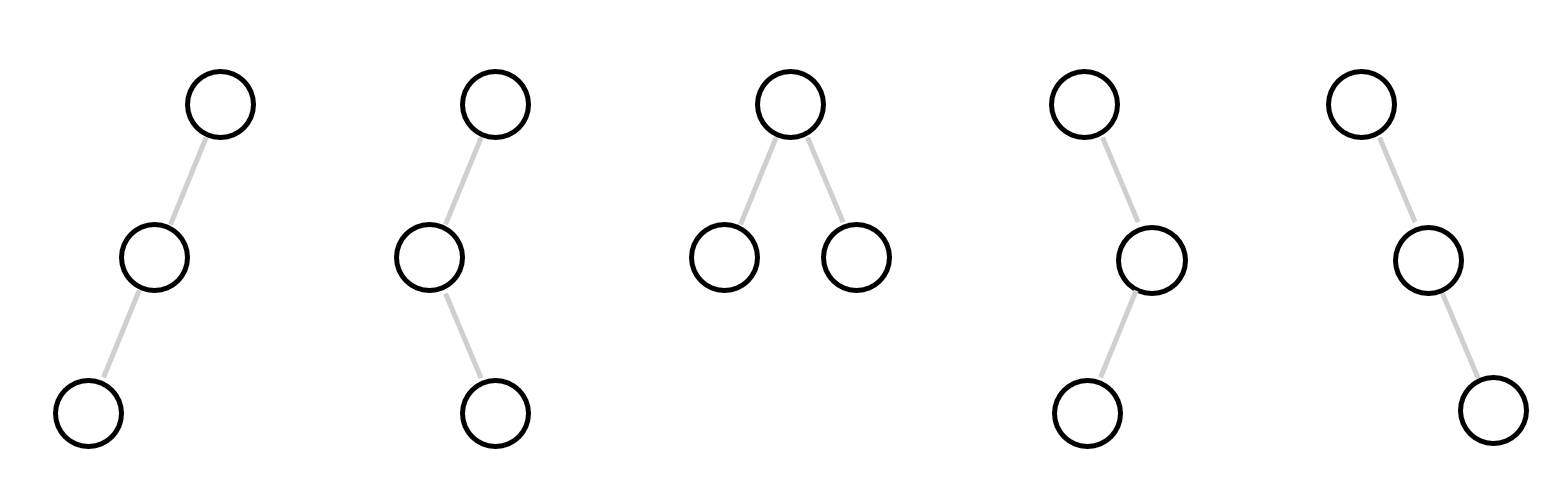
\includegraphics[width=\linewidth]{figures/TileShapes_Size3.PNG}
  \caption{All possible tile shapes with a tile size $n_t=3$}
  \label{Fig:TileSize3Shapes}
\end{figure}

\subsection{Valid Tiling of a Tree}
A tiling $\mathcal{T}$ of the tree $T = (V, E, r)$ with tile size $n_t$ is a partition $\{ T_1, T_2, ... ,T_m \}$ of the set $V$ such that 
\begin{enumerate}
    \item $T_1 \cup T_2 ... \cup T_m = V$
    \item $T_i \cap T_j = \emptyset$ for all $i, j \in [1, m]$ and $i \neq j$
    \item $|T_i| \leq n_t$ for all $i \in [1, m]$
    \item $\forall l \in L$ : $l \in T_i \rightarrow v \notin T_i \;\; \forall v \in V \backslash \{l\}$
    \item Tiles are \textbf{maximal}, i.e. if $|T_i| < n_t$, then there is no $v \in V\backslash \{ T_i \cup L \}$ such that $(u, v) \in E$ for some $u \in T_i$. 
    \item Tiles are \textbf{connected}, i.e. for an $u, v \in T_i$, there is a (undirected) path connecting $u$ and $v$ fully contained in $T_i$.
\end{enumerate} 

\TODO{AP We need to talk about how tiling is specified in the compiler}

\subsection{Tiled Trees}
A tiling transformation communicates the tiling to the Treebeard infrastructure by assigning a tile ID to each node in the decision tree. Using these tile IDs, Treebeard checks the validity of the tiling and then contructs a tree whose nodes are tiles. We call this tree the \textbf{\emph{tree of tiles}}. \TODO{We need a better name for this}
Figure \ref{Fig:ValidTilingTileSize3} shows a valid tiling with tile size 3 and the tree of tiles constructed by Treebeard. Three nodes are grouped into each of the tiles $t_1$ and $t_2$ as shown. Each tile is collapsed into a single node in the tree of tiles. However, each leaf in the original tree becomes a leaf in the tree of tiles.

\begin{figure}
  \centering
  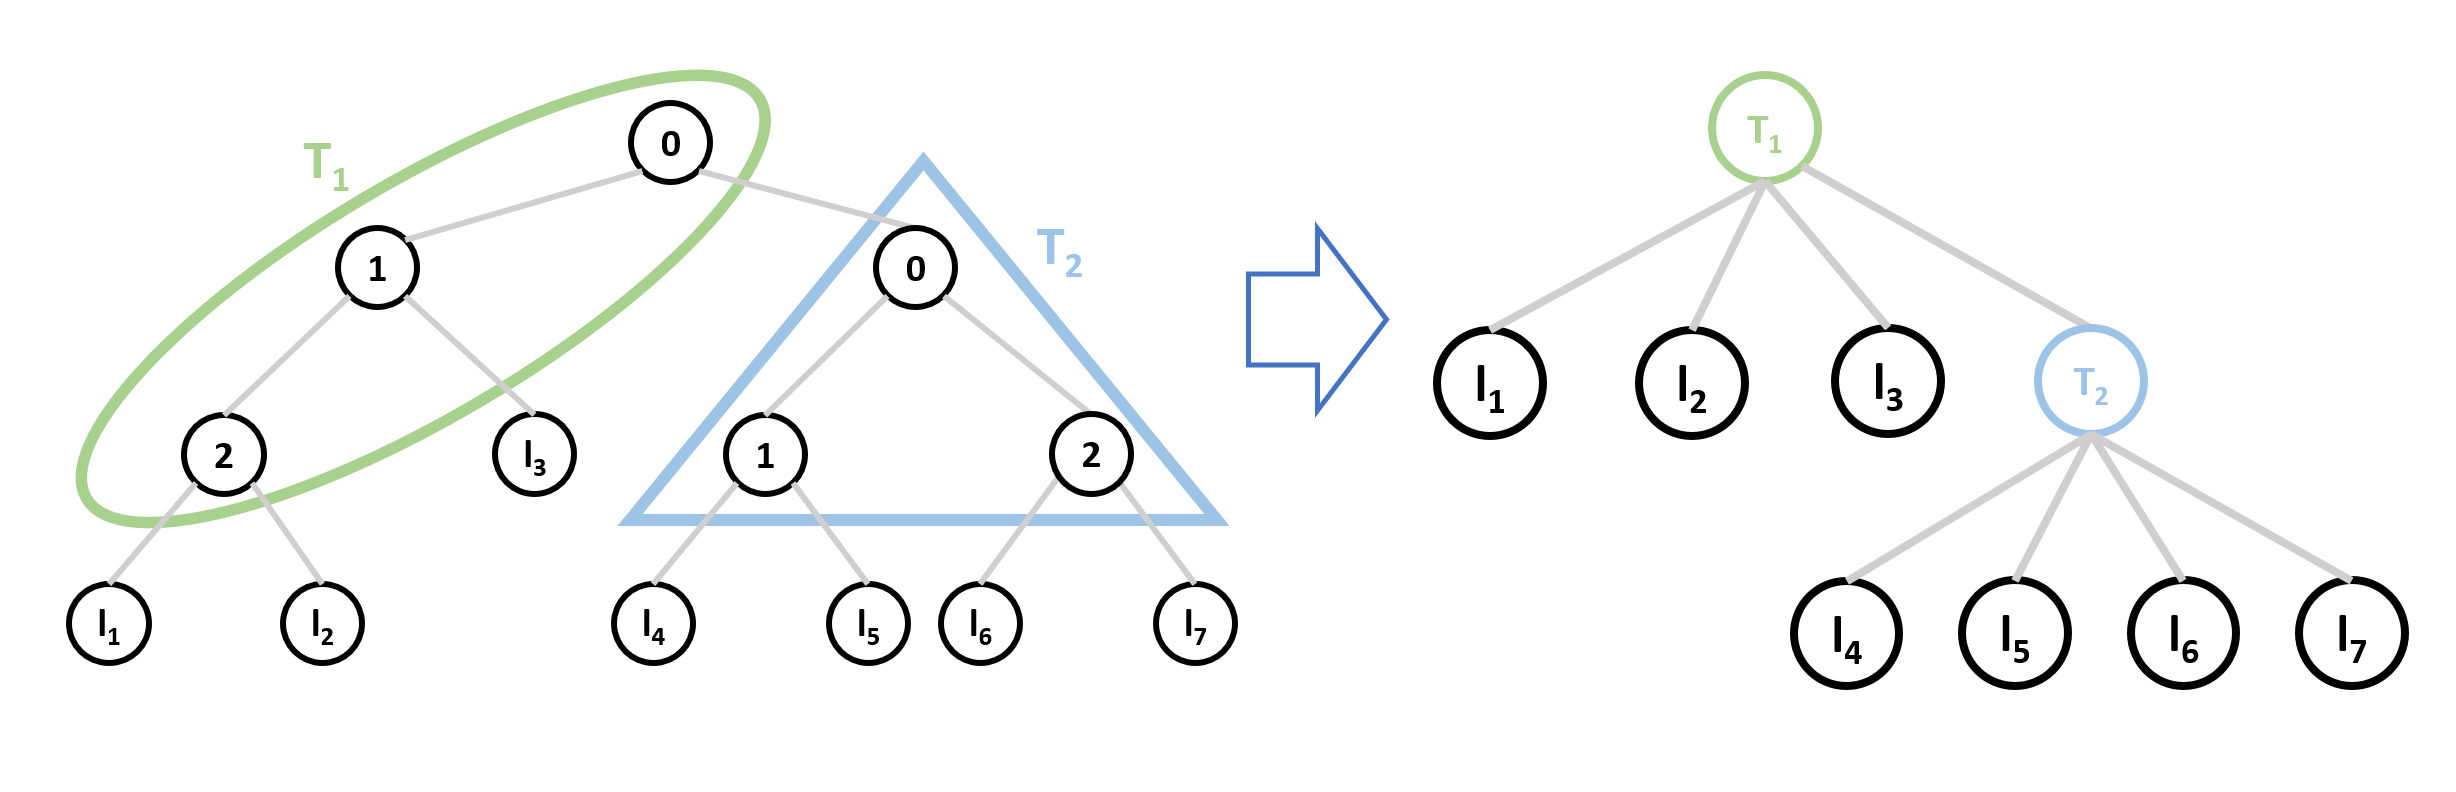
\includegraphics[width=\linewidth]{figures/TiledTree_Size3.PNG}
  \caption{Example of a valid tree tiling with a tile size $n_t=3$}
  \label{Fig:ValidTilingTileSize3}
\end{figure}

Treebeard maintains the following invariants.
\begin{enumerate}
  \item All tiles in a tree are the same size $n_t$. If the tiling produces any smaller tiles, these are padded by inserting dummy nodes to make them the required size.
  \item Nodes within tiles are always ordered in level order and left to right within a level. The numbering of the nodes in the above diagram shows this node order.
  \item Children of a node are numbered from left to right (regardless of level). For example, $l_1$ is the first child of $t_1$, $l_2$ is the second and so on.
\end{enumerate}
    
\subsection{Tile Shapes and Decision Tree Inference}
\label{Sec:TileShapesAndDecisionTreeInference}
Treebeard uses vector instructions to accelerate decision tree walks. Vector instructions are used to evaluate the predicates of all the nodes in a tile simultaneously. However, once the predicates of all the nodes in the tile are evaluated, computing the next tile to move to, given the outcome of the comparison depends on the tile shape of the current tile. To illustrate this problem, consider the case of the tiles of size 3 shown in figure \ref{Fig:TileTraversalTileSize3}. 
\begin{figure}
  \centering
  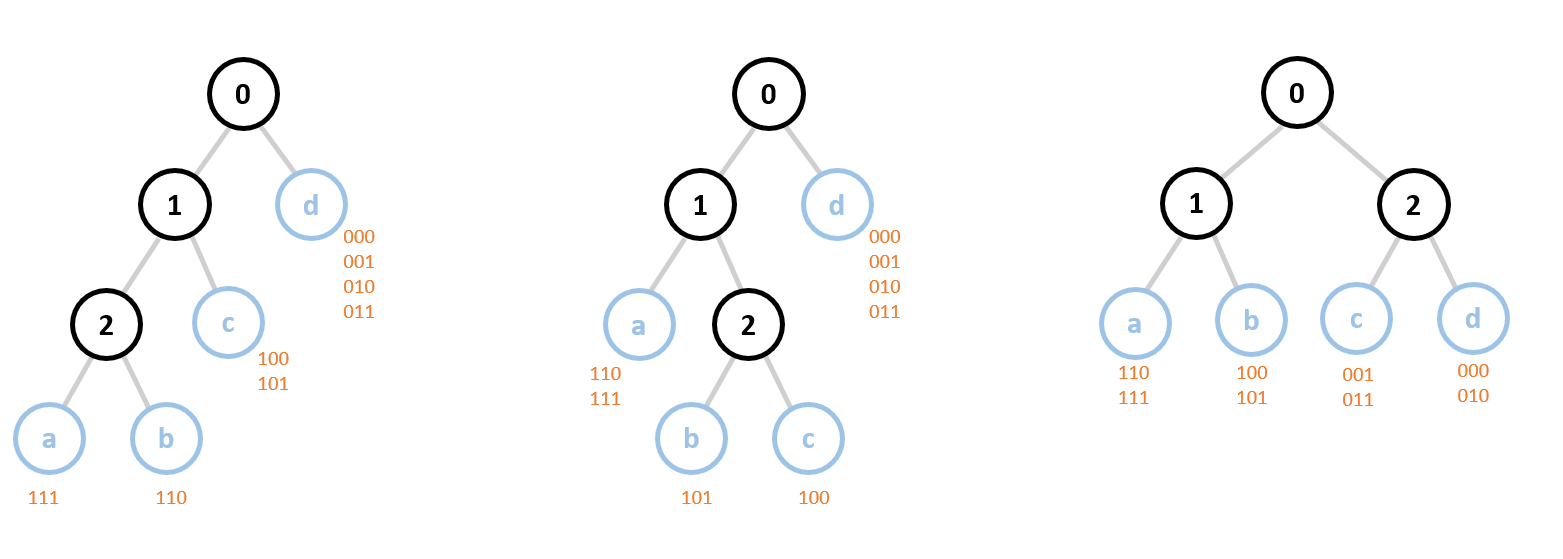
\includegraphics[width=\linewidth]{figures/TileTraversal_Size3.PNG}
  \caption{Example tile traversals with tile size $n_t=3$}
  \label{Fig:TileTraversalTileSize3}
\end{figure}
The diagram shows 3 of the 5 possible tile shapes for a tile size of 3. The nodes drawn in black are members of the tile $t_1$. The nodes in blue are the entry nodes of the children tiles of $t_1$. \TODO{Define entry nodes}

To traverse a tile on an input row, first, the predicate of each node in the tile is computed. Subsequently, we need to determine which of the child tiles to move to next. Note that a true predicte (bit value 1) on a node implies a move to the left child and a false predicate (bit value 0) implies a move to the right child.

In the diagram, the bit strings (written in red) show which child we need to move to given the outcomes of the comparison (the bits represent the comparison outcomes of nodes and are in the order of the nodes in the tile -- marked 0, 1 and 2 in the diagram, i.e., the MSB is the predicate outcome of node 0 and the LSB the predicate outcome of node 2). For example, for the first tile shape, if the predicate of all nodes are true (i.e. the comparison outcome is 111), the next node to evaluate is $a$. However, if the predicate of node 1 is false, then we need to move to $d$ regardless of the outcomes of nodes 2 and 3. It is easy to see from the diagram that, depending on the tile shape, the same predicate outcomes can mean moving to different children. For example, for the outcome "011", the next tile is the 4th child (node $d$) for the first two tile shapes while it is the 3rd child for the other tile shape (node $c$).

\subsection{Lookup Table}
A lookup table (LUT) is used to solve the problem described in section \ref{Sec:TileShapesAndDecisionTreeInference}, i.e. given the outcome of the comparisons on all nodes in a tile, determine the child tile we should evaluate next. The LUT is indexed by the tile shape and the comparison outcome. Formally, the LUT is a map.
\[
LUT : (TileShape, < Boolean \times n_t >) \rightarrow [0, n_t] \subset \mathbb{N}
\]

where $n_t$ is the tile size, $< Boolean \times n_t >$ is a vector of $n_t$ booleans. The value returned by the LUT is the index of the child of the current tile that should be evaluated next. For example, if we are evaluating the first tile $t$ in figure \ref{Fig:TileTraversalTileSize3}, and the result of the comparison is 110, then $LUT(TileShape(t), 110)=1$ since the tile we need to evaluate next is the tile with node $b$, which is the second child of the current tile.

In order to realize this LUT in generated code, Treebeard associates a non-negative integer ID with every unique tile shape of the given tile size. The result of the comparison, a vector of booleans, can be interpreted as a 64-bit integer. Therefore, the LUT can be implemented as a 2 dimensional array.
\begin{lstlisting}{style=c++}
  int16_t LUT[NTS(n_t), pow(2, n_t)]  
\end{lstlisting}

Treebeard computes the values in the LUT statically as the tile size is a compile time constant.

\subsection{In Memory Representation of Tiled Trees}
Treebeard currently has two in memory representations for tiled trees - an array based representation and a sparse representation. Both representations use an array of structs to represent all tiles of the model. 

\subsubsection{Array Based Representation}
\label{sec:ArrayBased}
Each tree in the model is represented as an array of tiles using the standard representation of trees as arrays. The root node is at index 0 and for a node at index $n$ in the array, the index of its $i^{th}$ child is given by $(n_t + 1) n + (i + 1)$ (every node in the tree of tiles has $n_t + 1$ children). A tile is represented by an object of the following struct.
\begin{lstlisting}{style=c++}
  struct Tile {
    // A vector of TileSize elements
    <ThresholdType x TileSize> thresholds; 
    <FeatureIndexType x TileSize> featureIndices;
    // Integer that identifies the tile shape
    TileShapeIDType tileShapeID; 
  };  
\end{lstlisting}
\TODO{AP Is this level of detail really needed? Also, the vector type notation needs to be introduced somewhere.}
Even though this representation is simple, the memory required for reasonable sized models is very large. The memory footprint is up to 20X that of the scalar representation. This memory bloat causes a performance degradation because the span of the L1 TLB is not sufficient to efficiently translate addresses for the whole model. \TODO{AP There are also some cache misses. Write this better.} Storing leaves as full tiles (even though leaves just have to represent one value) and the empty space introduced due to the array based representation of trees that are not complete account for most of the increase. The sparse representation described next tries to address these issues. 

\subsubsection{Sparse Representation}
\label{sec:SparseRep}
The sparse representation tries to address the large memory footprint of the array based representation by doing the following.

\begin{itemize}
  \item To eliminate the wasted space in the array representation, we add a child pointer to each tile. This points to the first child of the tile. All children of a tile are stored contiguously.
  \item Leaves are stored in a separate array. We found that, across all our benchmarks, a large fraction of leaves are such that all their siblings are also leaves. Such leaves are directly moved into the leaves array. For leaves for which this property does not hold, an additional hop is added by making the leaf tile a comparison tile and all its children are made leaves with the same value as the original leaf.
\end{itemize}

\begin{figure}
  \centering
  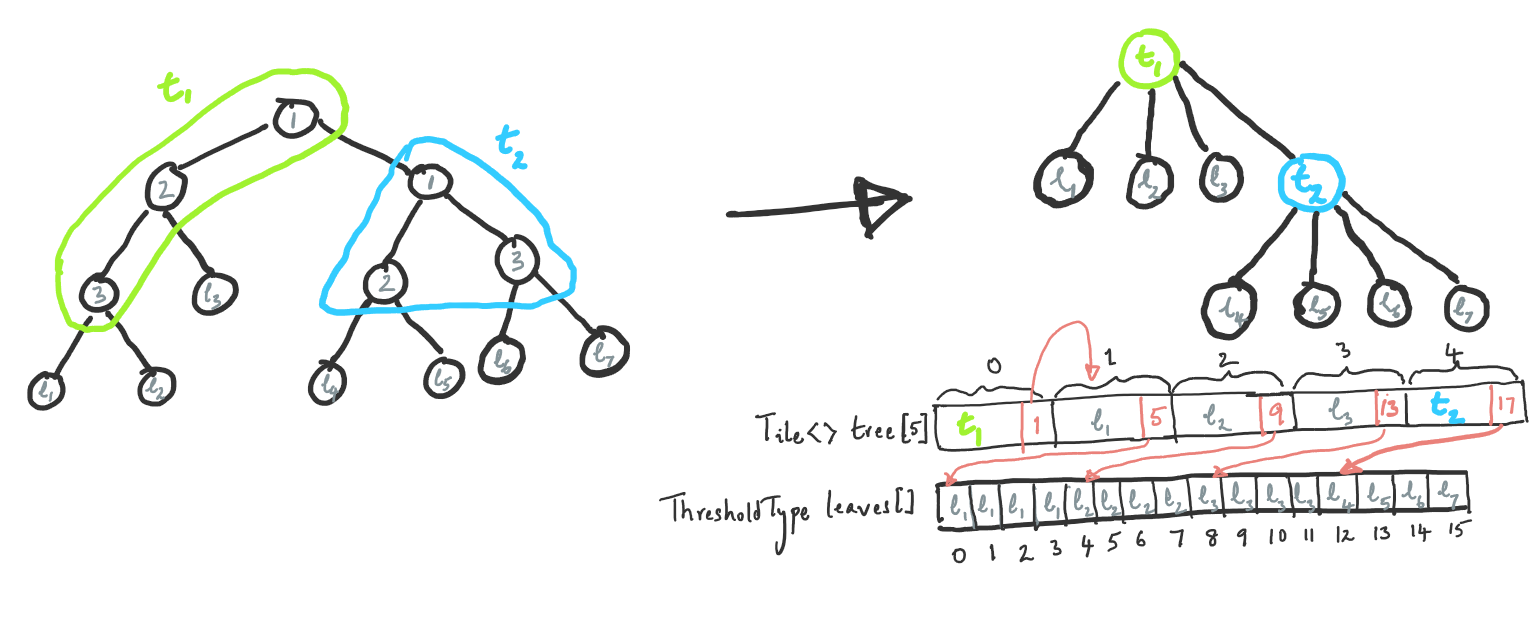
\includegraphics[width=\linewidth]{figures/SparseRep_TileSize3.PNG}
  \caption{Sparse representation with tile size $n_t=3$}
  \label{Fig:SparseRep}
\end{figure}

Figure \ref{Fig:SparseRep} shows some of the details of the sparse representation.
The tree on the left of the diagram is the actual decision tree with the nodes grouped into tiles $t_1$ and $t_2$. The tree on the right is the tree of tiles. The arrays depicted below show how the tree is represented in memory. The first array ($\texttt{tree}$) is an array of tiles and has 5 elements. Each element of the array represents a single tile and has the thresholds of the nodes, the feature indices, a tile shape ID and a pointer to the first child (shown explicitly in red). 

As a specific example, consider the tile $t_1$. The tile has four children -- $l_1$, $l_2$, $l_3$ and $t_2$ in that order (left to right). These tiles are stored contiguously in the $\texttt{tree}$ array and a pointer to the first of these, $l_1$ is stored in the tile $t_1$ (the index 1 is stored in the tile $t_1$ as shown). 

Now consider the tile $t_2$. Since all children of the tile $t_2$ are leaves, they are all moved into the $\texttt{leaves}$ array. To store a pointer into the $\texttt{leaves}$ array, we add $\texttt{len(tree)}$ to the element index in the $\texttt{leaves}$ array. The tile $t_2$'s child is the element at index 12 of the $\texttt{leaves}$ array. Therefore, the index $12 + 5 = 17$ is stored in the tile $t_2$. (Any index $i$ that is greater than the length of the $\texttt{tree}$ array is regarded as an index into the $\texttt{leaves}$ array. The index into the $\texttt{leaves}$ array is $i - \texttt{len(tree)}$.)

The other aspect of the representation is that an extra hop is added for the leaves $l_1$, $l_2$ and $l_3$ in order to simplify code generation. This enforces the invariant that all leaves are stored in the leaves array and  simplifies checking whether we've reached a leaf. Therefore, 4 new leaves are added as children for each of the original leaves $l_1$, $l_2$ and $l_3$. Each of these 12 newly added leaves has the same value as its parent. These are the first 12 elements of the $\texttt{leaves}$ array.

Even though we currently have implementations of the two representations detailed in sections \ref{sec:ArrayBased} and \ref{sec:SparseRep}, support for other representations is not hard to add. All optimizing passes that work on the high level and mid level IR will continue to work as is. Programmers need only provide new lowering passes for a few operations in the low level IR.
\subsection{Basic Tiling Algorithm}
\label{sec:UnifTiling}
% The justification for uniform tiling -- if we assume all paths are equally likely,
% we want to minimize the depth of speculation
Algorithm~\ref{Alg:UnifTilingAlgo} shows a simple tiling algorithm that satisfies all the above constraints. 
Tiling starts at the root and constructs a tile $Tile$ by performing
a level order traversal. The call \op{LevelOrderTraversal(r, $n_t$)} picks the next $n_t$ nodes according to the standard level order tree traversal algorithm (not described here) applied only to internal nodes of the tree. Once the current tile is constructed, the tiling procedure is recursively performed on all nodes that are 
destinations for edges going out of the constructed tile.
It is easy to see that the set of tiles constructed by algorithm \ref{Alg:UnifTilingAlgo} satisfies the constraints above.
\TODO{Pass a modified tree without leafs to the level order traversal call. Explicitly add leaves as seperate tiles}
% Algorithm for uniform tiling
\begin{algorithm}
  \caption{Uniform tree tiling}
  \label{Alg:UnifTilingAlgo}
  \begin{algorithmic}
      \Procedure{TileTree}{$tree = (V, E, r)$, $n_t$} 
          \If {$r \in L$}
              \State \textbf{return} $\{ r \}$
          \EndIf
          \State \textcolor{codegreen}{\textit{//Level order traversal to collect $n_t$ or fewer nodes. }}
          \State \textcolor{codegreen}{\textit{//Leaves are not included in the constructed tile. }}
          \State $Tile \leftarrow LevelOrderTraveral(r, n_t)$
          \State $Tiles =  \{ Tile \}$
          \For{$(u,v) \in Out(Tile)$}
              \State $Tiles \leftarrow Tiles \cup TileTree(S_v, n_t)$
          \EndFor
          \State \textbf{return} $Tiles$
      \EndProcedure
  \end{algorithmic}
\end{algorithm}

One interesting property of this tilling algorithm is that it naturally reduces the imbalance in trees, especially at large tile sizes. As the algorithm traverses down to sparser level of the tree, it naturally groups sub-trees containing chains of nodes, thus balancing the trees. While its possible to further enhance the algorithm to explicitly balance tiled trees, we find that basic tiling suffices in practice.
\CommentOut{
\subsubsection{Further Opimization and Code Generation}
We found that most leaf tiles for a given tree are at the same depth when uniform tiling is used. Furthermore, we see that deeper leaves 
are more likely to be reached.
%\footnote{Intuitively, this is true because training algorithms keep splitting nodes to maximize gain and gain
%will typically be maximized by splitting a large number of inputs.}.
Based on these observations, we (optionally) pad the tree of tiles generated with uniform tiling so that all leaves are at the same depth.
This transformation is performed on the high level IR after uniform tiling. 
Once the trees have been padded to make all leaves equal depth, the tree walks are fully unrolled to evaluate a fixed 
number of tiles and all leaf checks are omitted.

One other complication the code generator needs to handle is the fact that different trees in the model being 
compiled potentially have different depths. In order to handle
this, Treebeard sorts the trees by their depth. This ensures that all trees with equal depth are grouped together. Once this is done, 
the loop over the trees is fissed so that each of the resulting loops only walks trees of a single depth. Consider for example a 
forest with 4 trees $T_1$, $T_2$, $T_3$, and $T_4$ in that order. Further, assume that $T_1$ and $T_4$ have depth 2 while $T_2$ and $T_3$
have depth 3. First, Treebeard reorders the trees to be in the order $T_1$, $T_4$, $T_2$, $T_3$. Then, the loop over the trees is fissed
as shown in the following listing.

% loop transformations for uniform tiling (splitting) 
\begin{lstlisting}{style=c++}
  forest = ensemble(...)
  for i = 0 to batchSize step 1 {
    prediction = 0
    for t = 0 to 2 step 1 {
      tree = getTree(forest, t) 
      node = getRoot(tree)
      node = traverseTreeTile(tree, node, rows[i])
      treePrediction = getLeafValue(tree, node)
      prediction = prediction + treePrediction
    }
    for t = 2 to 4 step 1 {
      tree = getTree(forest, t) 
      node = getRoot(tree)
      node = traverseTreeTile(tree, node, rows[i])
      node = traverseTreeTile(tree, node, rows[i])
      treePrediction = getLeafValue(tree, node)
      prediction = prediction + treePrediction
    }
    predictions[i] = prediction
  }  
\end{lstlisting}

\TODO{AP: This listing is unnecesarily long. Can we maybe leave out the loop bodies and say something like "depth 2 walk"? Should 
we point to the figure in the overview section instead?}
}
\subsection{Probability Based Tiling}
\label{sec:ProbTiling}
%\subsubsection*{Motivation}

The next algorithm we propose exploits the inherent biases among the leaves of a decision tree. In typical machine learning models some leafs (equivalently outcomes or predictions) are more likely to be reached than others. In such settings, having balanced tiled trees is not sufficient to minimize expected inference time. 

Consider for example two machine learning models \op{airline-ohe} and \op{epsilon} (also used in our evaluation). 
Consider the graphs shown in   
figures \ref{Fig:AirlineOHEStats} and \ref{Fig:EpsilonStats} that are generated from training data. Each line in these graphs corresponds to a fixed fraction of the input (say $f$). 
A point on a line at coordinate $(x, y)$ means that a fraction $y$ of trees in the model could cover a fraction $f$ of all training inputs with a fraction $x$ of 
leaves. For example, the first point on the $f=0.9$ line in figure \ref{Fig:AirlineOHEStats} says that about 52\% of trees ($y$ value) need only 1\% of their
leaves ($x$ value) to cover 90\% of the training input. 
In general, Figure \ref{Fig:AirlineOHEStats} shows that very few leaves are needed to cover a very large fraction of inputs for the benchmark \op{airline-ohe}. 
This means that a small fraction of leaves are very likely. 
We call trees with a small number of extremely likely leaves \textbf{\emph{leaf biased}}.

On the other hand, for the benchmark \op{epsilon},
figure \ref{Fig:EpsilonStats} shows that a trees need a much larger fraction of their leaves to cover a significant fraction of the training input.
This means that most trees in \op{epsilon} are not leaf biased.

\CommentOut{
\subsubsection{More Notation}
In order to formulate the probability based tiling algorithm as an optimization problem, we define the following.
\begin{enumerate}
    \item For every leaf $l \in L$, we define $p_l$ as the probability that the leaf $l$ is reached.
    \item For each node $n \in V$, we define the absolute probability $p_v$ as
    \begin{equation}
        p_v = \begin{cases}
        p_l &\text{if $l \in L$}\\
        p_{left(v)} + p_{right(v)} &\text{otherwise}
        \end{cases}
    \end{equation}
    \item For any tree $T$, $\mathcal{C}(T)$ represents the set of all valid tilings of $T$.
    \item For every $v \in V$, we define $S_v$ as the subtree rooted at $v$.
    \item For every $v \in V$, we define $L_v$ as the set of leaves of $S_v$.
    \item For a every tile $T_i$, we define $root(T_i)$ as the node $v \in T_i$ such that $v$ has no incoming edges from any other node $u \in T_i$.
    \item For a tile $T_i$, $out(T_i) \subseteq E$ is the set of edges $(u, v)$ such that $u \in T_i$ and $v \notin T_i$.
\end{enumerate}
}

\begin{figure}
    \centering
    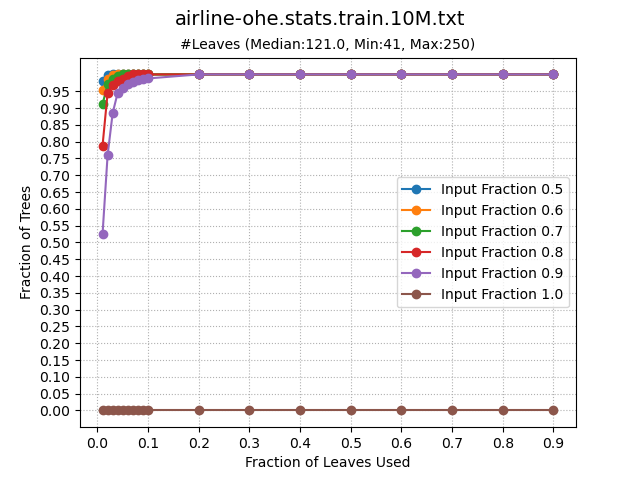
\includegraphics[width=\linewidth]{figures/airline-ohe.stats.train.txt.png}
    \caption{Statistical profile for airline-ohe}
    \label{Fig:AirlineOHEStats}
\end{figure}
\begin{figure}
    \centering
    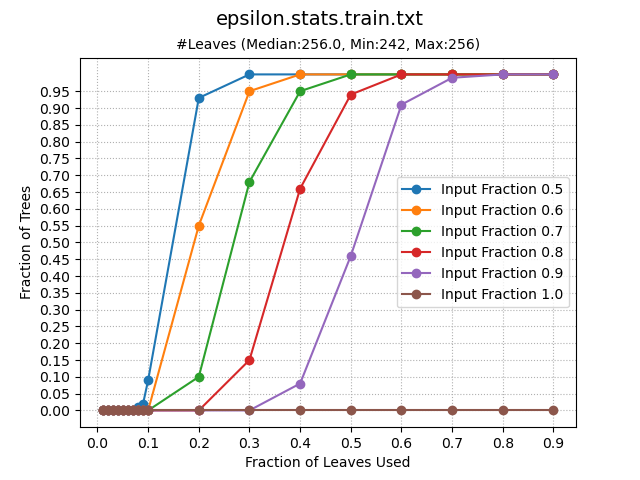
\includegraphics[width=\linewidth]{figures/epsilon.stats.train.txt.png}
    \caption{Statistical profile for epsilon}
    \label{Fig:EpsilonStats}
\end{figure}
\CommentOut{
We say that an input row $r_i$ is \textbf{\emph{covered}} by a subset of leaves $L' \subseteq L$ of a tree $T$, if the leaf $l$ reached by 
walking $T$ for row $r_i$ is in $L'$. We show how different models (and even different trees within the same model) behave differently 
using models for two benchmarks, airline-ohe and epsilon. Consider the graphs shown in   
figures \ref{Fig:AirlineOHEStats} and \ref{Fig:EpsilonStats}. Each line in these graphs corresponds to a fixed fraction of the input (say $f$). 
A point on a line at coordinate $(x, y)$ means that a fraction $y$ of trees in the model could cover a fraction $f$ of all training inputs with a fraction $x$ of 
leaves. For example, the first point on the $f=0.9$ line in figure \ref{Fig:AirlineOHEStats} says that about 52\% of trees ($y$ value) need only 1\% of their
leaves ($x$ value) to cover 90\% of the training input. 
In general, Figure \ref{Fig:AirlineOHEStats} shows that very few leaves are needed to cover a very large fraction of inputs for the benchmark airline-ohe. 
This means that a small fraction of leaves are very likely. On the other hand, for the benchmark epsilon,
figure \ref{Fig:EpsilonStats} shows that a trees need a much larger fraction of their leaves to cover a significant fraction of the test input.
This means that most trees in the epsilon model are not leaf biased.
One other observation we make is that most models have some leaf biased trees while the rest of the trees have equally likely leaves.
\TODO{AP Maybe define a term for trees with roughly equally likely leaves?} We design the probability based tiling algorithm to take advantage of this property 
of decision tree ensembles. 
}
\subsubsection{The Optimization Problem}

%We assume that we are given the probabilities of each leaf node of the decision tree (these can easily be computed using the training data). For every leaf $l \in L$, we %are given the probability $p_l$ that the leaf $l$ is reached. 

Observe that the latency of one tree walk is proportional to the number of tiles that need to be evaluated to reach the leaf. It is easy to see that for a leaf biased tree, basic tilling does not optimize for this objective, it considers all leafs to be equally likely. 
 
The goal of probablistic tiling is to minimize the average inference latency, or equivalently the minimize the expected number of tiles that are evaluated to compute one tree prediction. More formally, the problem is to find a \emph{valid} (as defined in Section~\ref{sec:ValidTiling}) tiling $\mathcal{T}$ such that the following objective is minimized.
\[
    \min_{\mathcal{T} \in \mathcal{C}(T)}{\sum_{l \in L_{\Tree}} p_l.depth_{\mathcal{T}}(l)}
\]
where the minimization is over all valid tilings $\mathcal{T}$ of the tree $\Tree$, $depth_{\mathcal{T}}(l)$ is the depth of the leaf $l$ given tiling ${\mathcal{T}}$. $p_l$ is the probability of of reaching leaf $l$ as observed during training.

The above optimization problem can be solved optimally using dynamic programming. 
We leave this out in the interest of space. 
Instead, we use the simple greedy algorithm listed in algorithm \ref{Alg:GreedyTilingAlgo} to construct a valid tiling given the node probabilities\footnote{Probabilites for internal nodes can be computed from probablities for leafs by summing up the probabilities of all leafs that belong to the sub-tree rooted at the internal node. Leaf probabilities are collected during training.}.
The algorithm starts at the root and greedily keeps adding the most probable legal node to the current tile until the maximum tile size is reached.
Subsequently, the tiling procedure is recursively performed on all nodes that are destinations for edges going out of the constructed tile.

% \subsubsection{Dynamic Programming Formulation}


% For any node $v \in V$, we define
% \[
%     cost(v, \mathcal{T}) = \sum_{l \in L_v} p(l | v).depth_{\mathcal{T}}(l)
% \]
% where $\mathcal{T} \in \mathcal{C}(T_v)$.

% Then, the objective function, for the tree $T_v$, can be rewritten as 
% \[
%     opt\_cost(v) = \min_{\mathcal{T} \in \mathcal{C}(T_v)}{cost(v, \mathcal{T})}
% \]

% The objective function can then be rewritten in the following recursive form.
% \[
%     opt\_cost(v) = \min_{T_0 \in TileShapes(n_t, v)}{1 + \sum_{(n_1, n_2) \in out(T_0)} p(n_1 | v)p(n_2 | n1)opt\_cost(n_2)}
% \]
% where $TileShapes(n_t, v)$ is the set of all tile shapes of size $n_t$ with root $v$. A straight forward substitution argument shows why the solution to the subproblems (tiling all sub-trees) needs to to be optimal. The objective is now in a form that can solved using
% dynamic programming. 

% \subsubsection{Greedy Algorithm}

% Intuitively, it seems like the following greedy algorithm also gives the optimal tiling. The algorithm starts at the root and greedily keeps adding the most probable node to the current tile until the maximum tile size is reached.
\begin{algorithm}
    \caption{Greedy Probability Based Tree Tiling}
    \label{Alg:GreedyTilingAlgo}
    \begin{algorithmic}
        \Procedure{TileTree}{$\Tree = (V, E, r)$, $n_t$} 
            \If {$r \in L_{\Tree}$}
                \State \textbf{return} $\{ r \}$
            \EndIf
            \State $Tile \leftarrow \{ r \}$
            \While{$|Tile| < n_t$}
                \State $e = (u,v) \in Out(Tile)$ st $p(v)$ is max and $v \notin L$
                \If{$e = \emptyset$}
                    \State \textbf{break}
                \EndIf
                \State $Tile = Tile \cup \{ v \}$
            \EndWhile
            \State $Tiles =  \{ Tile \}$
            \For{$(u,v) \in Out(Tile)$}
                \State $Tiles \leftarrow Tiles \cup TileTree(S_v, n_t)$
            \EndFor
            \State \textbf{return} $Tiles$
        \EndProcedure
    \end{algorithmic}
\end{algorithm}

% Talk about problems with increasing number of tile shapes and only performing such tiling on skewed trees
\CommentOut{
When we tried to apply algorithm \ref{Alg:GreedyTilingAlgo} on all trees in our benchmarks, we found
that even minor variations in probability caused the tiling algorithm to generate a large 
number of tile shapes. This in turn caused a loss in performance because the large size of the 
lookup table needed (section \ref{sec:LookupTable}) caused increased L1 cache misses. In order to 
alleviate this, we only perform probability based tiling on trees that are leaf biased.
}
We find probability based tiling is only beneficial for leaf biased trees\footnote{Turns out that for trees that are not leaf biased, probability based tiling produces many more tile shapes (see Section~\ref{sec:tileShapes}) which direclty impacts the cost of \op{getChildTile} making it more expensive than basic tiling.}.  Recall that   
a tree to be leaf biased if a small fraction of leaves, say $\alpha$, can cover a large fraction of training inputs, say $\beta$.
We only perform probability based tiling on trees with thresholds $\alpha=0.05$ and $\beta=0.9$ and fall back to uniform tiling otherwise. 




\subsection{Unroll and Jam}
While tiling and subsequent vectorization gives significant performance gains, profiling 
the generated code showed that true dependencies between instructions were still causing
a significant number of stall cycles. In order to fill these stall cycles, Treebeard does 
an unroll and jam on the inner most loops of the loop nest. This transformation has 
the effect of walking multiple tree and input row pairs in an interleaved fashion. 
The dependency stalls can be hidden by scheduling instructions from independent tree walks 
in the stall cycles. 

This optimization is performed across both the mid-level IR and low-level IR. Loops on which 
to perform unroll and jam are identified in the mid-level IR. This information is communicated to the 
lowering passes by replacing these tree walks with specialized tree walk operations. The lowering 
passes that transform the mid-level IR to low-level IR interleave operations across independent
tree walks.

The following listing shows the mid-level IR when the inner loop over the input rows is unrolled 
by a factor of 2 and the two resulting tree walks are jammed together.

\begin{lstlisting}[style=c++]
  forest = ensemble(...)
  for t = 0 to 4 step 1 {
    for i = 0 to 2 step 2 {
      tree = getTree(forest, t)
      prediction1, prediction2 = InterleavedWalk((tree, rows[i]), (tree, rows[i+1]))
    }
  }
\end{lstlisting}

When lowered to low-level IR, the operations to traverse each of the tree, input row pairs 
(the arguments to the \texttt{InterleavedWalk}) are interleaved. One step of the interleaved 
walk is listed below. 
\begin{lstlisting}[style=c++]
  // ... 
  n1 = n2 = getRoot(tree)
  // ...
  threshold1 = loadThresholds(n1)
  threshold2 = loadThresholds(n2)
  featureIndex1 = loadFeatureIndices(n1)
  featureIndex2 = loadFeatureIndices(n2)
  feature1 = rows[i][featureIndex1]
  feature2 = rows[i][featureIndex2]
  pred1 = feature1 < threshold1
  pred2 = feature2 < threshold2
  n1 = getChildNode(n1, pred1)
  n2 = getChildNode(n2, pred2)
  // ...
\end{lstlisting}
These transformations are fairly general and are not aware of the in memory representation of the model. Therefore, they 
are reusable across different in memory representations - the ones that are currently built into Treebeard or ones that 
are added in the future.
\TODO{AP I feel the way this section is currently written makes the optimization seem extremely trivial. Is there a different 
way to present it?}
\subsection{Vectorization}
\label{sec:Vectorization}
Vectorization performed by Treebeard is enabled by the tiling transformations described in section \ref{sec:Tiling}. 
When the low level IR is translated to LLVM IR, Treebeard generates LLVM instructions that operate on the threholds and feature indices 
of nodes within a tile in a vector fashion. Therefore, thresholds and feature indices are loaded using vector loads and predicates are 
evaluated using vector comparisons. These vector LLVM IR instructions are then converted to vector instructions in the target ISA by 
the LLVM JIT.

The below listing shows some of the details of a vectorized tree walk. 
\begin{lstlisting}[style=c++]
  // A lookup table that determines the child index of
  // the next tile given the tile shape and the outcome
  // of the vector comparison on the current tile
  int16_t LUT[NUM_TILE_SHAPES, pow(2, TileSize)]
  
  ResultType Prediction_Function(...) {
    // ...
    Node n = getRoot(tree)
    while (isLeaf(tree, n)==false) do {
      thresholds = loadThresholds(tree, n)
      featureIndices = loadFeatureIndices(tree, n)
      // Gather required feature from the current row
      features = rows[i][featureIndices]
      // Vector comparison of features and thresholds
      comparison = features < thresholds
      
      // Pack bits in comparison vector into an integer
      comparisonIndex = combineBitsIntoInt(comparison)
      
      // Get child index of tile we need to move to
      tileShape = loadTileShape(tree, n)
      childIndex = LUT[tileShapeID, comparisonIndex]
      
      // Move to the correct child of the current node
      n = getChildNode(tree, n, childIndex) 
    }
    ThresholdType prediction = getLeafValue(n)
    // ...
  }  
\end{lstlisting}
To evaluate the current tile, the vector of thresholds is first loaded (\texttt{loadThresholds}). This vector contains the thresholds of all nodes in the tile. Then, the features required for comparison are gathered into a vector (lines 11 and 13). The feature vector is compared to the threshold vector and the child tile to move to is determined (lines 15 to 25). More details about tile shapes and the look up table are presented in subsequent sections.

\subsubsection{Tile Shapes}
Informally, the \textbf{\emph{tile shape}} is the shape of the region that encloses all nodes in a tile in a diagram of the decision tree. More formally, for a tile size $n_t$, each unique legal binary tree containing $n_t$ nodes (nodes being indistinguishable) corresponds to a tile shape.

Figure \ref{Fig:TileSize3Shapes} enumerates all tile shapes with a tile size of 3. There are a total of 5 tile shapes with size 3. The number of tile shapes with a tile size $n_t$, denoted by $NTS(n_t)$ is given by the following equation. 

\begin{equation}
  NTS(n) = \sum_{k=0}^{n-1} NTS(k) \times NTS(n-k-1)
\end{equation}

where $NTS(0) = NTS(1) = 1$.

\begin{figure}
  \centering
  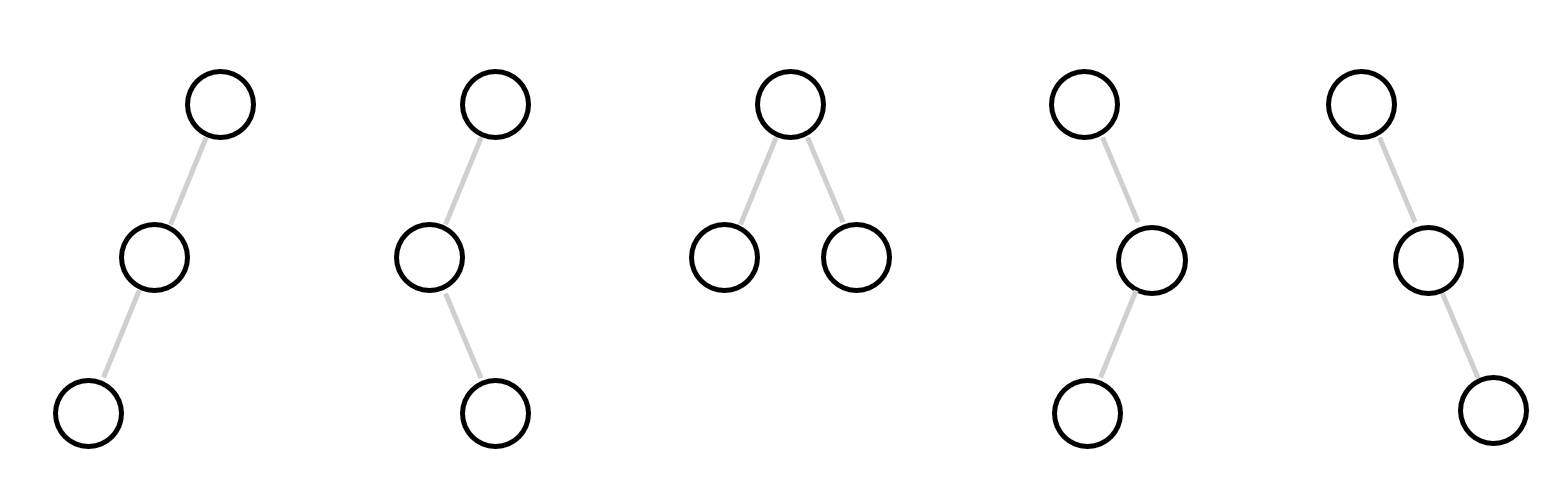
\includegraphics[width=\linewidth]{figures/TileShapes_Size3.PNG}
  \caption{All possible tile shapes with tile size $n_t=3$}
  \label{Fig:TileSize3Shapes}
\end{figure}

\subsubsection{Tile Shapes and Decision Tree Inference}
\label{Sec:TileShapesAndDecisionTreeInference}
Treebeard uses vector instructions to accelerate decision tree walks. Vector instructions are used to evaluate the predicates of all the nodes in a tile simultaneously. However, once the predicates of all the nodes in the tile are evaluated, computing the next tile to move to, given the outcome of the comparison depends on the tile shape of the current tile. To illustrate this problem, consider the case of the tiles of size 3 shown in figure \ref{Fig:TileTraversalTileSize3}. 
\begin{figure}
  \centering
  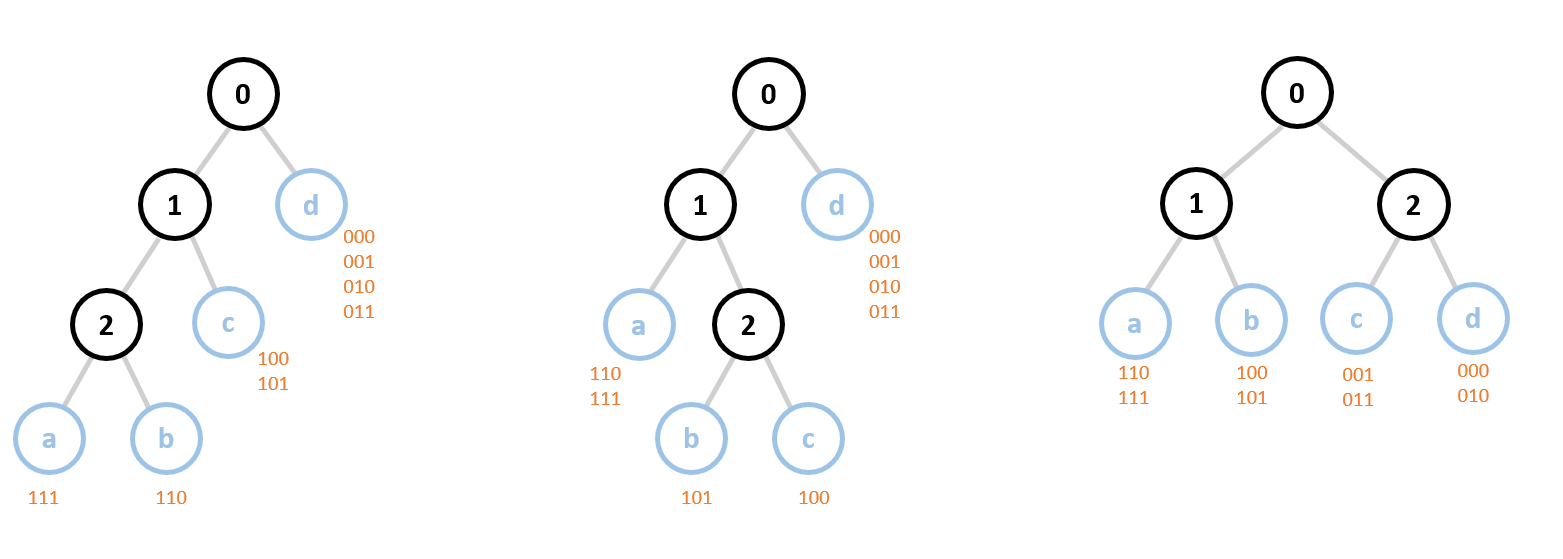
\includegraphics[width=\linewidth]{figures/TileTraversal_Size3.PNG}
  \caption{Example tile traversals with tile size $n_t=3$}
  \label{Fig:TileTraversalTileSize3}
\end{figure}
The diagram shows 3 of the 5 possible tile shapes for a tile size of 3. The nodes drawn in black are members of the tile $t_1$. The nodes in blue are the entry nodes of the children tiles of $t_1$. \TODO{Define entry nodes}

% To traverse a tile on an input row, first, the predicate of each node in the tile is computed. Subsequently, we need to determine which of the child tiles to move to next. Note that a true predicte (bit value 1) on a node implies a move to the left child and a false predicate (bit value 0) implies a move to the right child.

In the diagram, the bit strings (written in red) show which child we need to move to given the outcomes of the comparison. The bits represent the comparison outcomes of nodes and are in the order of the nodes in the tile -- marked 0, 1 and 2 in the diagram, i.e., the MSB is the predicate outcome of node 0 and the LSB the predicate outcome of node 2. For example, for the first tile shape, if the predicates of all nodes are true (i.e. the comparison outcome is 111), the next node to evaluate is $a$. 
% However, if the predicate of node 1 is false, then we need to move to $d$ regardless of the outcomes of nodes 2 and 3.
It is easy to see from the diagram that, depending on the tile shape, the same predicate outcomes can mean moving to different children. For example, for the outcome "011", the next tile is the 4th child (node $d$) for the first two tile shapes while it is the 3rd child for the other tile shape (node $c$).

\subsubsection{Lookup Table}
\label{sec:LookupTable}
A lookup table (LUT) is used to solve the problem described in section \ref{Sec:TileShapesAndDecisionTreeInference}, i.e. given the outcome of the comparisons of all nodes in a tile, determine the child tile we should evaluate next. The LUT is indexed by the tile shape and the comparison outcome. Formally, the LUT is a map.
\[
LUT : (TileShape, < Boolean \times n_t >) \rightarrow [0, n_t] \subset \mathbb{N}
\]

where $n_t$ is the tile size, $< Boolean \times n_t >$ is a vector of $n_t$ booleans. The value returned by the LUT is the index of the child of the current tile that should be evaluated next. For example, if we are evaluating the first tile $t$ in figure \ref{Fig:TileTraversalTileSize3}, and the result of the comparison is 110, then $LUT(TileShape(t), 110)=1$ since the tile we need to evaluate next is the tile with node $b$, which is the second child of the current tile.

In order to realize this LUT in generated code, Treebeard associates a non-negative integer ID with every unique tile shape of the given tile size. The result of the comparison, a vector of booleans, can be interpreted as a 64-bit integer. Therefore, the LUT can be implemented as a 2 dimensional array.
% \begin{lstlisting}{style=c++}
%   int16_t LUT[NTS(n_t), pow(2, n_t)]  
% \end{lstlisting}
Treebeard computes the values in the LUT statically as the tile size is a compile time constant.
\TODO{AP What comes after subsubsection?}

\subsection{In Memory Representation of Tiled Trees}
Treebeard currently has two in memory representations for tiled trees - an array based representation and a sparse representation. Both representations use an array of structs to represent all tiles of the model. 

\subsubsection{Array Based Representation}
\label{sec:ArrayBased}
Each tree in the model is represented as an array of tiles using the standard representation of trees as arrays. The root node is at index 0 and for a node at index $n$ in the array, the index of its $i^{th}$ child is given by $(n_t + 1) n + (i + 1)$ (nodes in the tree of tiles have $n_t + 1$ children). A tile is represented by an object of the following struct.
\begin{lstlisting}{style=c++}
  struct Tile {
    // A vector of TileSize elements
    <ThresholdType x TileSize> thresholds; 
    <FeatureIndexType x TileSize> featureIndices;
    // Integer that identifies the tile shape
    TileShapeIDType tileShapeID; 
  };  
\end{lstlisting}
\TODO{AP Is this level of detail really needed? Also, the vector type notation needs to be introduced somewhere.}
Even though this representation is simple and efficient for small models, the memory required for bigger models is very large. 
%The memory footprint is up to 20X that of the scalar representation.
This memory bloat causes performance problems because the span of the L1 TLB is not sufficient to efficiently translate 
addresses for the whole model. Storing leaves as full tiles (even though leaves just have to represent one value) and the
empty space introduced due to the array based representation of trees that are not complete account for most
of the increase.
%The sparse representation described next tries to address these issues. 

\subsubsection{Sparse Representation}
\label{sec:SparseRep}
The sparse representation tries to address the large memory footprint of the array based representation by doing the following.

\begin{itemize}
  \item We add a child pointer to each tile to eliminate the wasted space in the array representation. This points to the first child of the tile. All children of a tile are stored contiguously.
  \item Leaves are stored as a separate array of scalar values. Across all our benchmarks, after tiling a large fraction of 
  leaves are such that all their siblings are also leaves. Such leaves are directly moved into the leaves array. For leaves
  for which this property does not hold, an extra ``hop'' is added by making the original leaf tile a normal tile. All its
  children are made leaves with the same value as the original leaf.
\end{itemize}

\begin{figure}
  \centering
  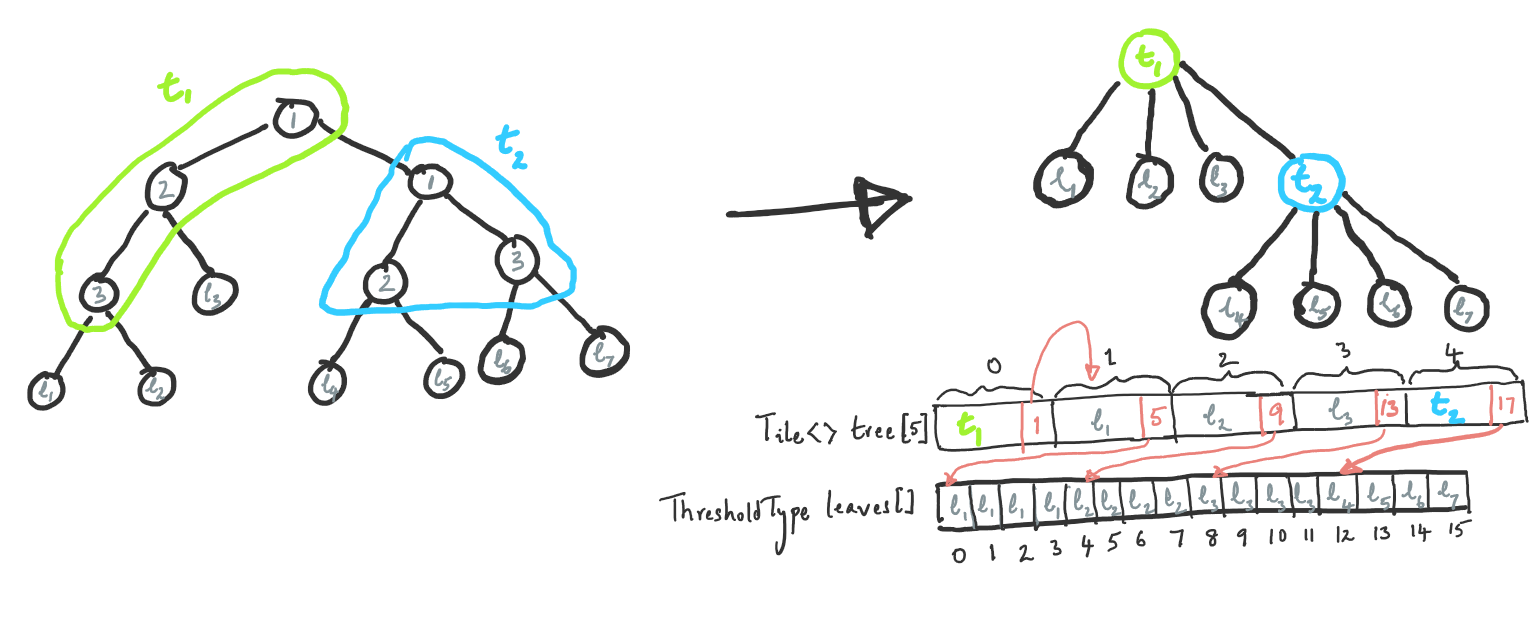
\includegraphics[width=\linewidth]{figures/SparseRep_TileSize3.PNG}
  \caption{Sparse representation with tile size $n_t=3$}
  \label{Fig:SparseRep}
\end{figure}

Figure \ref{Fig:SparseRep} shows some of the details of the sparse representation.
% The tree on the left of the diagram is the actual decision tree with the nodes grouped into tiles $t_1$ and $t_2$. The tree on the right is the tree of tiles.
The arrays depicted below show how the tree is represented in memory. The first array ($\texttt{tree}$) is an array of tiles 
and has 5 elements. Each element of the array represents a single tile and has the thresholds of the nodes, the feature
indices, a tile shape ID and a pointer to the first child (shown explicitly in red). 

As a specific example, consider the tile $t_1$. The tile has four children -- $l_1$, $l_2$, $l_3$ and $t_2$ in that order (left to right). These tiles are stored contiguously in the $\texttt{tree}$ array and a pointer to the first of these, $l_1$ is stored in the tile $t_1$ (the index 1 is stored in the tile $t_1$ as shown). 

Now consider the tile $t_2$. Since all children of the tile $t_2$ are leaves, they are all moved into the $\texttt{leaves}$ array.
To store a pointer into the $\texttt{leaves}$ array, we add $\texttt{len(tree)}$ to the element index in the $\texttt{leaves}$ array.
The tile $t_2$'s child is the element at index 12 of the $\texttt{leaves}$ array. Therefore, the index $12 + 5 = 17$ is stored in 
the tile $t_2$. Any index $i$ that is greater than the length of the $\texttt{tree}$ array is regarded as an index into the
$\texttt{leaves}$ array. The index into the $\texttt{leaves}$ array is $i - \texttt{len(tree)}$.

The other aspect of the representation is that an extra hop is added for the leaves $l_1$, $l_2$ and $l_3$ in order to simplify
code generation. This enforces the invariant that all leaves are stored in the leaves array and  simplifies checking whether
we've reached a leaf. Therefore, 4 new leaves are added as children for each of the original leaves $l_1$, $l_2$ and $l_3$. 
Each of these 12 newly added leaves has the same value as its parent. These are the first 12 elements of the $\texttt{leaves}$ array.

Even though we currently have implementations of the two representations detailed in sections \ref{sec:ArrayBased} 
and \ref{sec:SparseRep}, support for other representations is not hard to add. All optimizing passes that work on 
the high level and mid level IR will continue to work as is. Programmers need only provide new lowering passes for
a few operations in the low level IR.

\subsubsection{Code Generation for Probability Based Tiling}
As probability based tiling pulls the most probable leaves of a decision tree nearest the root, it poses 
some implementation challenges. By design, the tiling process makes the tree of tiles 
imbalanced. The array based representation (section \ref{sec:ArrayBased})
cannot be used because of the memory footprint increase (a large part of the tree is empty, but would need to be allocated).
On the other hand, the sparse representation in section \ref{sec:SparseRep} adds 
an extra hop for leaves that have non-leaf siblings. But this would mean that we add extra hops for 
the most probable leaves after probability based tiling which defeats the optimization.

We address these challenges using a code generation strategy. Treebeard peels 
the tree walk and specializes the leaf checks at higher levels to avoid the extra hop. Currently, 
we determine the maximum depth of leaves needed to cover 90 percent of the inputs and peel the tree 
walk by as many iterations. For example, consider the case where leaves until depth 2 are needed to 
cover 90 percent of the training input. Then, Treebeard generates the following IR. 

\begin{lstlisting}{style=c++}
    // ...
    tree = getTree(forest, t)
    node = getRoot(tree)
    node = traverseTreeTile(tree, node, rows[i])
    if (isLeafTile(node)) {
        treePrediction = getLeafValue(tree, node)
    } else {    
        node = traverseTreeTile(tree, node, rows[i])
        if (isLeafTile(node)) {
            treePrediction = getLeafValue(tree, node)
        } else {    
            // Loop based traversal 
        }
    }
    treePrediction = getLeafValue(tree, node)
    // ...
\end{lstlisting}

The if statements check whether a node is a leaf tile and hence avoid the extra hop. 
%The memory 
%requirement is also not increased because only a small fraction of leaves are represented as full tiles.
While walk peeling is used to improve the performance of probability based tiling by specializing leaf tests,
the transformation is by itself general and can be used in different contexts. For example, it could be used 
to elide leaf checks until a depth $d$ is reached if we know all leaves are at a depth greater than $d$. 

One other issue that the code generator needs to handle is that walks of different trees in the same ensemble may 
need to be peeled to different depths. A strategy similar to what is used for uniform tiling is used to handle this.
Trees are reordered so that all trees 
with equal peeling depth are grouped together and the loops in the IR are fissed so that tree walks 
for these groups of trees can be specialized differently.
% This is very similar to the code generation strategy used for uniform tiling.


\subsection{Parallelization}
Currently, Treebeard performs a naive parallelization of the inference computation. When parallelism is enabled, the 
loop over the input rows is parallelized using OpenMP. Treebeard rewrites 
the mid-level IR by tiling the loop over the input rows with a tile size equal to the number of cores. 
As a concrete example, consider the case where we intend to perform inference using a model with 4 trees 
on a batch of 64 rows. Further, assume that we wish to parallelize this computation across 8 cores. 
Treebeard then generates the following IR.
\begin{lstlisting}[style=c++]
  forest = ensemble(...)
  parallel.for i0 = 0 to 64 step 8 {
    for i1 = 0 to 8 step 1 {
      i = i0 + i1
      prediction = 0
      for t = 0 to 4 step 1 {
        tree = getTree(forest, t) 
        treePrediction = WalkTree(tree, rows[i])
        prediction = prediction + treePrediction
      }
      predictions[i] = prediction
    }
  }
\end{lstlisting}
Currently, as our focus is on single core performance, we do not 
do any parallelism related optimizations (such as loop tiling). We leave a more thorough exploration of parallelization 
to future work.